\documentclass[twoside, letterpaper, 12pt]{report}
\usepackage{orthodoxservicebook}

\title{The Sunday Reader's Service of the \\ \textsc{Typica} \\ 2020 May 03}
\titlepic{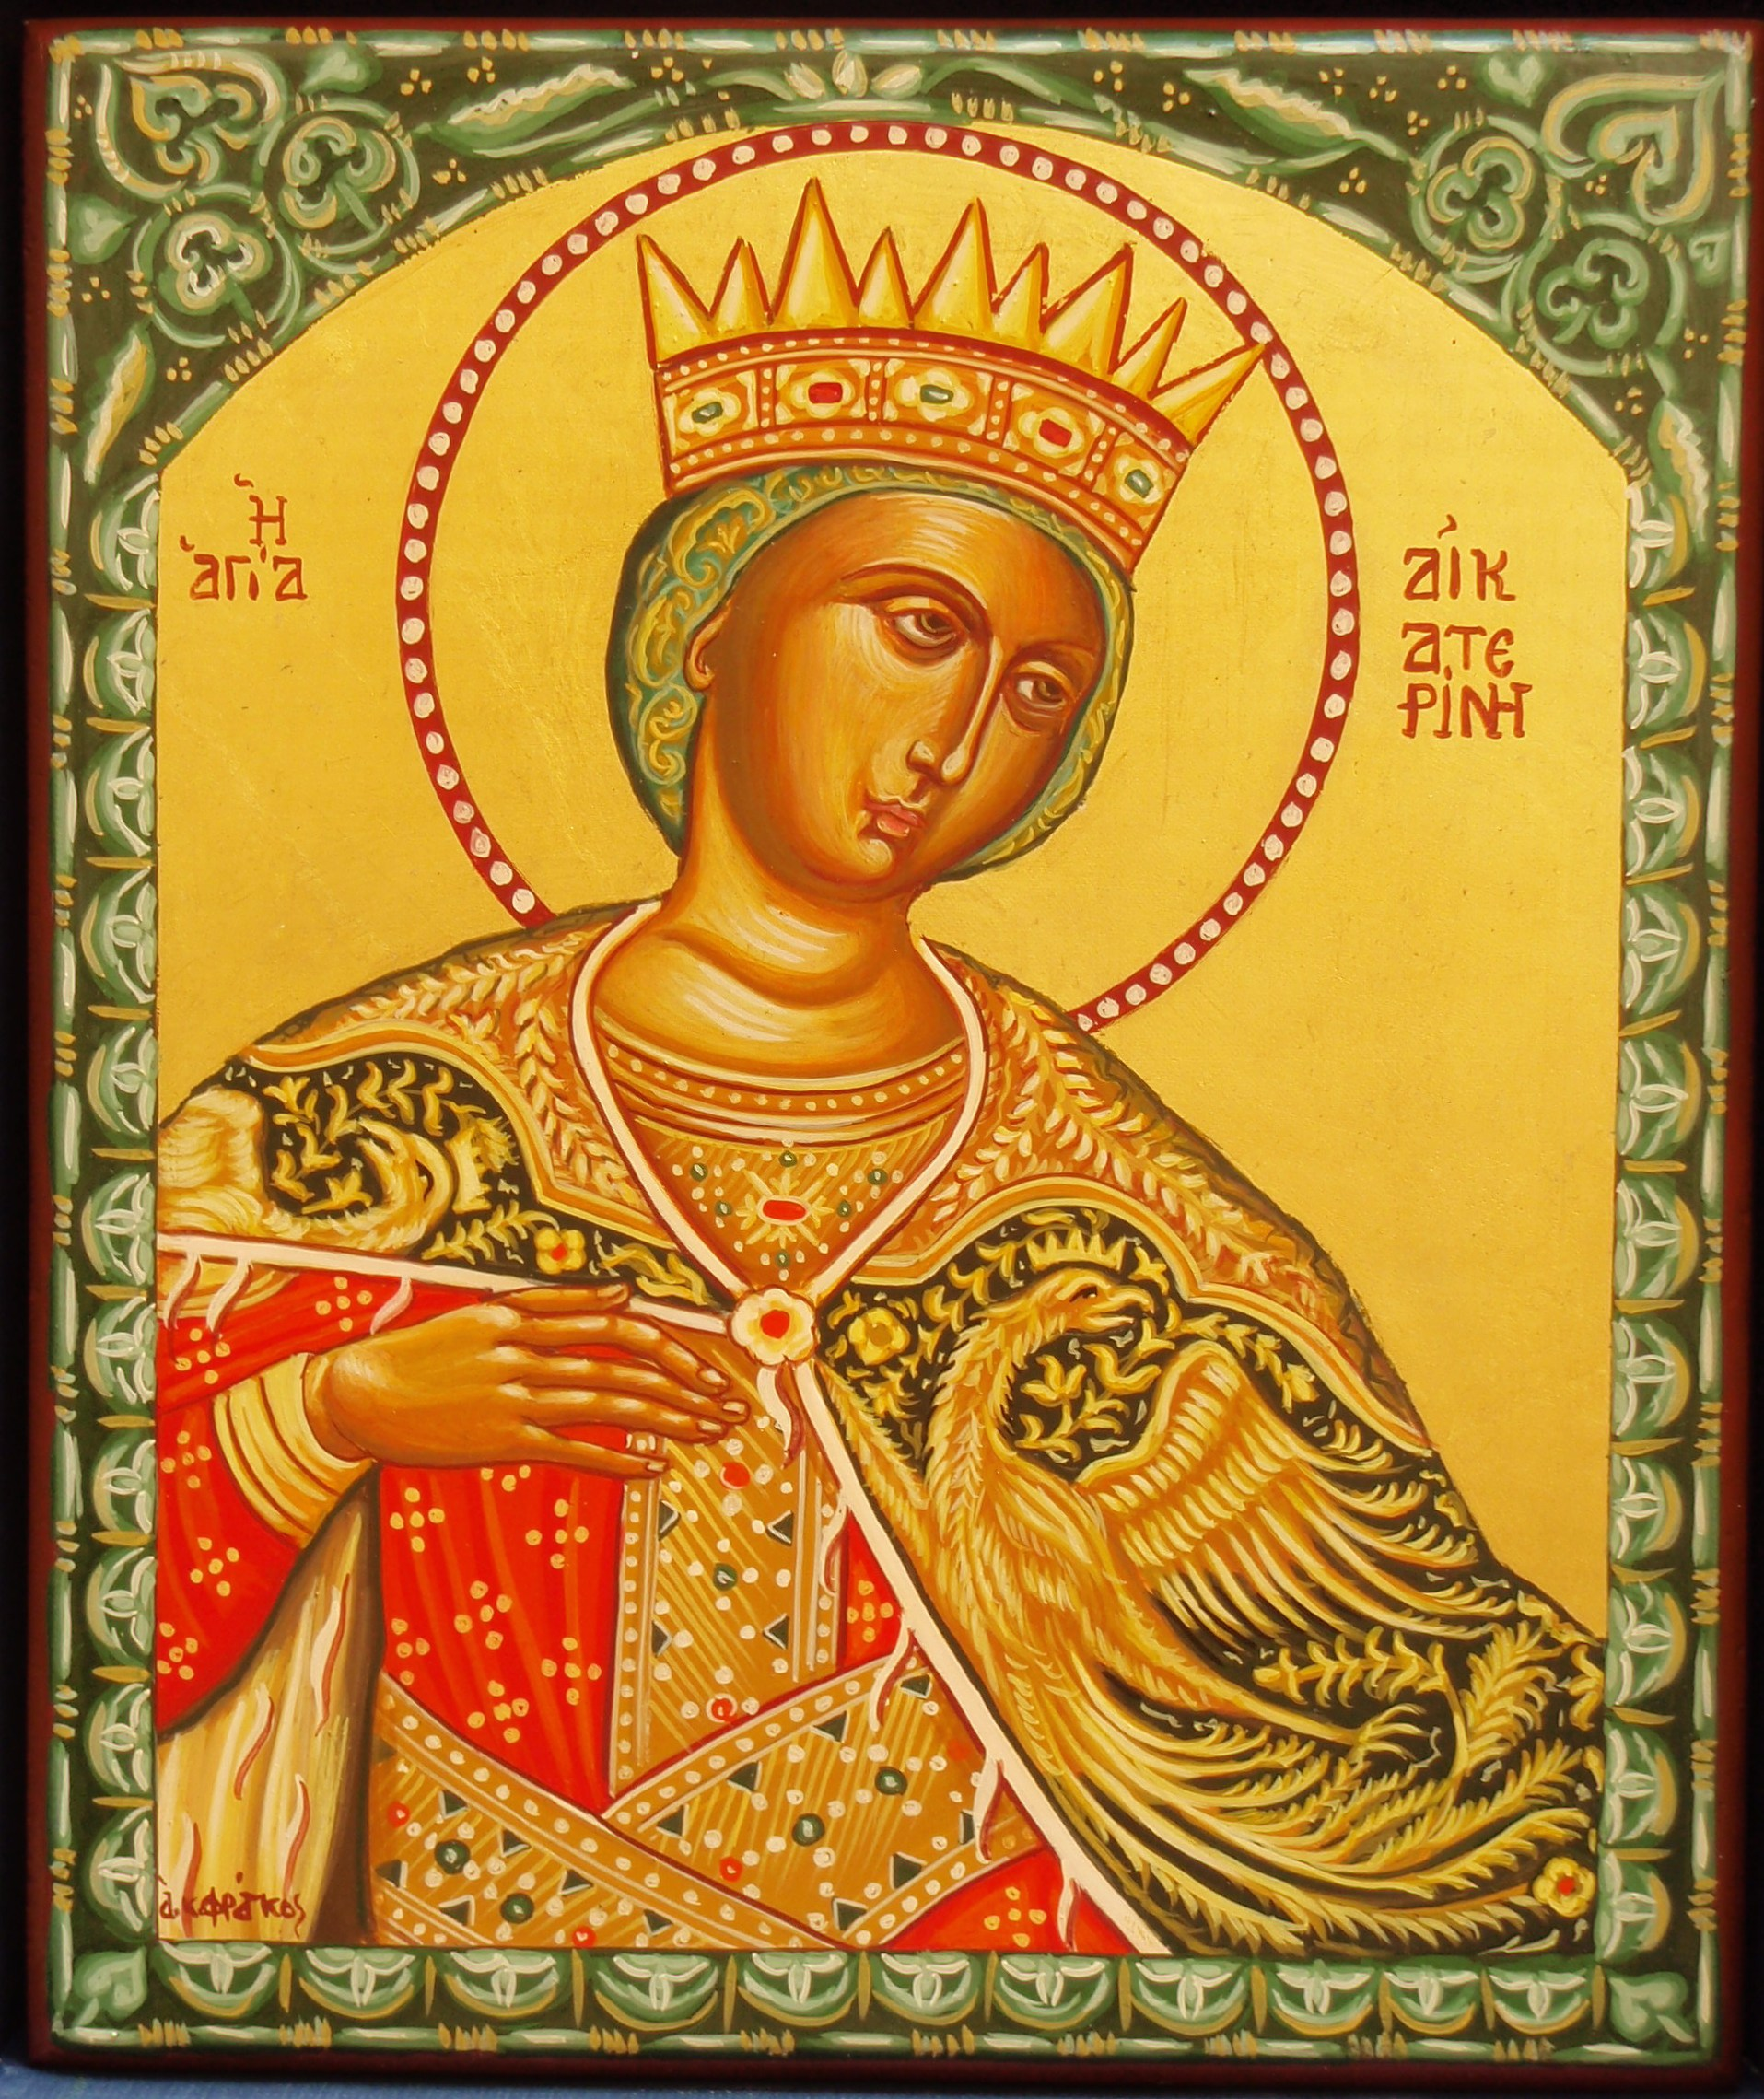
\includegraphics[width=0.5\textwidth]{Katherine1.jpg}}
\date{}
\author{}

\begin{document}
\maketitle
\pagestyle{empty} % Don't show page numbers
\instruction{This page intentionally left blank}
\cleardoublepage
\pagestyle{plain}
\setcounter{page}{1} % Set the page counter to 1 on the first real page
\chapter*{Service of Typica on Sunday, May 03}
\instruction{Sunday of the Myrrh-Bearing Women, Pious Joseph of Arimathaea
  \& Righteous Nicodemus}

\readerline{\throughtheprayers{}}
\choralresponse{./Z-Responses/Obikhod/Amen.ly}

\trisagionNeedsAmen[reader][prepentecost]

\choralresponse{./Z-Responses/Obikhod/Amen.ly}


\centeredsection{The First Antiphon}
\lilypondfile{./Liturgy/B-FirstAntiphon/BlessTheLord_Greek-Music.ly}

\centeredsection{The Second Antiphon}
\lilypondfile{./Liturgy/C-SecondAntiphon/PraiseTheLord_Greek-Music.ly}

\centeredsection{The Third Antiphon}
\lilypondfile{./Liturgy/D-ThirdAntiphon/Beatitudes_Moscow-Music.ly}

\centeredsection{The Epistle}

\instruction{Both of the New Testament lessons are read
without liturgical introduction or conclusion.
The readers start with “The Reading from…” and proceeds}

\paragraph{The Reading from the Acts of the Saintly and Pure Apostles. (6:1-7)}\mbox{}\\

\begin{maybetwocolumns}
In those days, when the disciples were increasing in number, the Hellenists murmured
against the Hebrews because their widows were neglected in the daily distribution. And the Twelve
summoned the body of the disciples and said, “It is not right that we should give up preaching the
word of God to serve tables. Therefore, brethren, pick out from among you seven men of good
repute, full of the Spirit and of wisdom, whom we may appoint to this duty. But we will devote
ourselves to prayer and to the ministry of the word.” And what they said pleased the whole
multitude, and they chose Stephen, a man full of faith and of the Holy Spirit, and Philip, and
Prochorus, and Nicanor, and Timon, and Parmenas, and Nicolaos, a proselyte of Antioch. These
they set before the apostles, and they prayed and laid their hands upon them. And the word of God
increased; and the number of the disciples multiplied greatly in Jerusalem, and a great many of the
priests were obedient to the faith.
\end{maybetwocolumns}

\centeredsection{The Gospel}

\instruction{Both of the New Testament lessons are read
without liturgical introduction or conclusion.
The readers start with “The Reading from…” and proceeds}

\paragraph{The Reading from the Holy Gospel according to St. Mark. (15:43-16:8)}\mbox{}\\

\begin{maybetwocolumns}
At that time, Joseph of Arimathaea, a respected member of the council, who was also
himself looking for the Kingdom of God, took courage and went to Pilate, and asked for the body
of Jesus. And Pilate wondered if He were already dead; and summoning the centurion, he asked
him whether Jesus was already dead. And when he learned from the centurion that He was dead,
he granted the body to Joseph. And he bought a linen shroud, and taking Him down, wrapped Him
in the linen shroud, and laid Him in a tomb, which had been hewn out of the rock; and he rolled a
stone against the door of the tomb. Mary Magdalene and Mary the mother of Joses saw where He
was laid. And when the Sabbath was passed, Mary Magdalene, Mary the mother of James, and
Salome, bought spices so that they might go and anoint Him. And very early on the first day of the
week they went to the tomb when the sun had risen. And they were saying to one another, “Who
will roll away the stone for us from the door of the tomb?” And looking up, they saw that the stone
was rolled back— it was very large. And entering the tomb, they saw a young man sitting on the
right side, dressed in a white robe; and they were amazed. And he said to them, “Do not be amazed;
you seek Jesus of Nazareth, Who was crucified. He has risen, He is not here; see the place where
they laid Him. But go, tell His Disciples and Peter that He is going before you to Galilee; there
you will see Him, as He told you.” And they went out and fled from the tomb; for trembling and
astonishment had come upon them; and they said nothing to anyone, for they were afraid.
\end{maybetwocolumns}

\centeredsection{Troparia Before the Creed}
\instruction{Plain reading}
\begin{reader}
\item[Reader 1:] The heavenly choir singeth thy praises, saying:
  Holy, holy, holy, Lord of Sabaoth; heaven and earth are full of Thy glory.

\item[Reader 2:] \emph{Come unto him, and be enlightened,
               and your faces shall not be ashamed.}
  The heavenly choir singeth thy praises, saying:
  Holy, holy, holy, Lord of Sabaoth; heaven and earth are full of Thy glory.

\item[Reader 1:] \emph{\glory}
  The choir of the holy angels and archangels,
  with all the powers of heaven, singeth thy praises, saying:
  Holy, holy, holy, Lord of Sabaoth; heaven and earth are full of Thy glory.

\item[Reader 2:]\emph{\nowandever}
\end{reader}

\centeredsection{The Creed}
\input{Common/TheCreed.txt}


\centeredsection{Prayer of Forgiveness}
\readerline{Forgive, remit, pardon, O God, our sins,
  both voluntary and involuntary, in deed and in word, in knowledge or in ignorance,
  committed by night or by day, in mind and in thought.
  Forgive us them all, for thou art good and lovest mankind.
}


\centeredsection{The Lord’s Prayer}
\input{Common/LordsPrayer.txt}

\readerline{Through the prayers of our holy fathers, Lord Jesus Christ our God, have mercy on us.}
\choralresponse{./Z-Responses/Obikhod/Amen.ly}


\centeredsection{Kontakia for Pascha in Tone 8}
\lilypondfile{./Pentecostarion/Pascha/Pascha-Kontakion-T8-Byz-Karam-Music.ly}

\readerline{\lhmForty}

\readerline{
  O Christ our God, Who art worshipped and glorified at all times at every hour both in
  heaven and on earth; Who art long-suffering and plenteous in mercy and compassion; Who lovest
  the just man and showest mercy upon the sinner; and Who callest all men to repentance through 
  the promise of blessings to come; receive, O Lord, at this very hour our supplications, and direct
  our lives in the way of Thy commandments: sanctify our souls, purify our bodies, set our minds
  aright, cleanse our thoughts; deliver us from all affliction, trouble, and distress; compass us about
  with Thy holy angels, that, guided and guarded by them, we may attain unto the unity of the Faith,
  and to the knowledge of Thine unapproachable glory; for Thou art blessed unto ages of ages. Amen.
}

\begin{reader}
  \item \lhmThree{}\\\emph{\gne{}}
  \item \morehonorablethanthetherubim{}
  \item \throughtheprayers{}
\end{reader}

\begin{maybetwocolumns}
\choralresponse{./Z-Responses/Obikhod/Amen.ly}

\readerline{\blessedbethename{}\thrice{}}

\centeredsection{Psalm 33}
\input{./Psalms/Psalm033-unknowntrans.txt}

\centeredsection{Psalm 144}
\input{./Psalms/Psalm144-unknowntrans.txt}
\end{maybetwocolumns}

\peopleline{\gne}


\centeredsection{A Homily}
\begin{maybetwocolumns}
\instruction{Second Sunday after Pascha, 7th Sunday of Quarantine\\
With a Courage Born of Love:\\
Homily for the Sunday of the Myrrh Bearing Women in the Orthodox Church\\
Fr. Philip LeMasters, pastor, St. Luke Antiochian Orthodox Church of Abilene, Texas}

Christ is Risen! We have now been celebrating our Lord’s victory over death for two
weeks. We will continue to do so for a few more weeks, saying, “Christ is Risen” many times.
But we must not let our celebration of Pascha stop there. For we want to live the new life that the
Lord has brought to the world; we want to participate in His victory over sin, death, and all that
separates us from life eternal. And we can learn an important lesson in how to do that from those
who were at the empty tomb on Easter morning as the first witnesses of the resurrection to hear
the word of the angel: “He is Risen. He is not here… Go tell His disciples—and Peter—that He
is going before you to Galilee; there you will see Him, as He said to you.”

These first witnesses of our salvation were women who went to the tomb with oil and spices to
anoint the dead body of Jesus Christ. They obviously did not expect the tomb to be empty. They
were surely heart-broken, afraid, and terribly disappointed that their Lord had been killed. But
they had the strength to offer Him one last act of love: to anoint His body properly for burial. Just
imagine the risks that they took, publicly identifying themselves with the Lord at His crucifixion
and then going to the tomb of One executed as a traitor in the wee hours of Sunday morning. With
a courage born of love, they must have put aside obvious concerns about their personal safely. And
as they did so, these women– Mary the Theotokos, Mary Magdalene, two other Mary’s, Johanna,
Salome, Martha, Susanna and others whose names we do not know– received the greatest news
in the universe, the resurrection of our Lord, God, and Savior Jesus Christ. Yes, the angelic
proclamation of Pascha came first to the Theotokos, even as she was the first to hear from the
Archangel the good news of the Incarnation.

As you will remember, the male disciples did not believe their testimony at first, even as St. Joseph
the Betrothed was at first skeptical of the circumstances of the Lord’s virgin conception. But with
the balance between man and woman that we see throughout the unfolding of our salvation, we
remember along with these blessed women two men: Ss. Joseph of Arimathaea and Nicodemus,
prominent Jewish leaders who were also secret followers of Jesus Christ. This Joseph risked his
position and possibly his life by asking Pilate for the Savior’s body, even as Joseph the Betrothed
had surely risked his life during the flight to Egypt to escape the persecution of the wicked King
Herod. Nicodemus, who had understood the Lord so poorly in a conversation recorded near the
beginning of St. John’s gospel, came to faith and joined Joseph of Arimathaea in wrapping the
Lord in linen with spices and placing Him in a tomb.

Like the myrrh-bearing women, these men must have been terribly sad and afraid. Their hopes
had been cruelly crushed; their world turned upside down. Not only had their Lord died, He was
the victim of public rejection, humiliation, and capital punishment. Nonetheless, these women and
men did what had to be done, despite the risk to themselves from the authorities and their own
pain. They served their Christ in the only way still available to them by caring for His body.

Before Jesus Christ’s death, He washed the feet of His disciples in order to show them what it
meant to serve in humility as He did. The myrrh-bearers were not present that evening, but they
followed the Lord’s example of service better than anyone else. Perhaps they were not there
because they had already learned the centrality of humble service in how they cared for and
supported the Lord throughout His ministry. Regardless, their selfless devotion to Christ put them
in the place where they would be the first to receive the good news of the resurrection, the first to
share in the joy of Pascha. We have a lot to learn from them, as well as from Joseph and
Nicodemus. For if we want to live the new life of our Lord’s victory over death and corruption in
all its forms, we must do as they did by serving our Lord in humility out love, despite the cost.

We have no lack of opportunities to serve Christ, in His Body, the Church: whether by visiting the
sick, giving of our time and other resources to the poor, providing someone without transportation
a ride to church, maintaining our building and grounds, cleaning and beautifying the church
temple, teaching Sunday School, chanting, hosting coffee hour, baking holy bread, serving on the
parish council or at the altar, reading the epistle in liturgy, inviting others to visit our services, or
otherwise doing what needs to be done for the flourishing of our parish. These things may seem
small, but they make a huge difference. If we are not faithful in small tasks, how can we hope to
be faithful in large ones? Out of love for Christ, let us all answer the call to serve Him as we are
needed in His Body, the Church.

We are also reminded of the importance of humble service by today’s passages from Acts in which
the first deacons were ordained to oversee the distribution of bread to the needy widows who were
supported by the Christian community. The word deacon means “servant,” and we read that, after
the deacons began their ministry, “the word of God spread, and the number of the disciples
multiplied greatly in Jerusalem and a great many of the priests were obedient to the faith.” Perhaps
the passage reads that way because humble service is the very backbone of the Church, an essential
part of our faithfulness and growth as Christ’s Body.

Of course, we do not encounter the Lord only in the visible boundaries of the Church. For every
human being is an icon of Christ, especially the poor, needy, and miserable. In that we care for
the least of these in society, for prisoners or refugees or the lonely or mentally ill, we care for Him.
In that we neglect them, we neglect Him. The myrrh-bearers did not disregard Christ’s body in
the tomb, and neither should we disregard the Lord’s body hungry, sick, poorly clothed, abused,
or otherwise suffering in our world. It is not hard to find the Lord in people we encounter every
day who need our service and attention. That is why we should all bring our Lenten collections for
“Food for Hungry People” to church as soon as we can. And food, clothing, and other items
brought to church will always be put to good use by those who need them, regardless of the season
of the year.

On this Sunday of the Myrrh-Bearing Women, it is clear that holiness is not a matter of earthly
power or prestige. Those righteous women did not count for much at all in their time and place;
even the male disciples disregarded their preaching of the resurrection. The new day of God’s
reign ushered in by Pascha is a passing over from spiritual blindness, self-centeredness, and
domination to love, selfless service, and true humility before God and all who bear His image and
likeness. Here we encounter the same apparent weakness manifest in our Lord’s cross, which
ultimately destroyed the corrupt orders of our distorted world through the glory of the empty tomb.
If we want to participate even now in that glory, if we want to embrace a power beyond the powers
of this age, we must follow the example of those courageous and loving women and men who
risked their lives out of love for our Lord, God, and Savior Jesus Christ. No, a life of courageous
love for our Savior is not easy, but it is the only path that we lead us to behold, and even to
participate personally in, the good news of His resurrection on the third day, which is ultimately
what this blessed season is all about.

\end{maybetwocolumns}

\centeredsection{Ressurrectional Apolytikion in Tone 2}
\lilypondfile{./Octoechos/ResurrectionalApolytikion-Tone2-Kazan-Music.ly}

\centeredsection{Apolytikion of Joseph of Arimathaea in Tone 2}
The noble Joseph, taking Thine immaculate Body down from the Tree, and having wrapped It in
pure linen and spices, laid It for burial in a new tomb. But on the third day Thou didst arise, O
Lord, granting to the world Great Mercy

\centeredsection{Apolytikion of the Myrrh-Bearing Women in Tone 2}
Unto the myrrh-bearing women did the Angel cry out as he stood by the grave: Myrrh-oils are
meet for the dead, but Christ hath proved to be a stranger to corruption. But cry out: The Lord is
risen, granting to the world Great Mercy.


\readerline{\throughtheprayers}

\choralresponse{./Z-Responses/Obikhod/Amen.ly}

\end{document}

